\documentclass[aspectratio=169]{beamer}
\usepackage{UFtheme}
%_______________________________________________
\usepackage{tikz}
\usetikzlibrary{shapes,arrows,positioning}
\tikzset{decision/.style={diamond, draw, fill=blue!20, text width=4.5em, text badly centered, inner sep=0pt}}
\tikzset{block/.style={rectangle, draw, fill=blue!20, text width=7em, text centered, rounded corners,
 minimum width=3.5cm}}
\tikzset{line/.style={draw, -latex}}
%_______________________________________________

\title{ \textbf{\textcolor{red}{WRLib}} --- A C++ library for solving PDEs with space-time parallel algorithms\vspace{1cm}}
\author{ Pankaj K Mishra, Felix Kwok}
\institute{Department of Mathematics, Hong Kong Baptist University}
\date{\today}
%% ===========================================
%% ===========================================
\begin{document}
\begin{frame}[plain]
    \titlepage
\end{frame} 
%% ===========================================
%% ===========================================

% Uncomment these lines for an automatically generated outline.
%\begin{frame}{Outline}
%  \tableofcontents
%\end{frame}


%% ===========================================
%% ===========================================
%	PRESENTATION SLIDES
%% ===========================================
%% ===========================================

%% ===========================================
%% ===========================================
\section{First Section} 
\subsection{Subsection Example} 
%% ===========================================

\begin{frame}
\frametitle{\normalsize Step 1 --- Geometry}
\begin{center}
\scalebox{0.6}{
      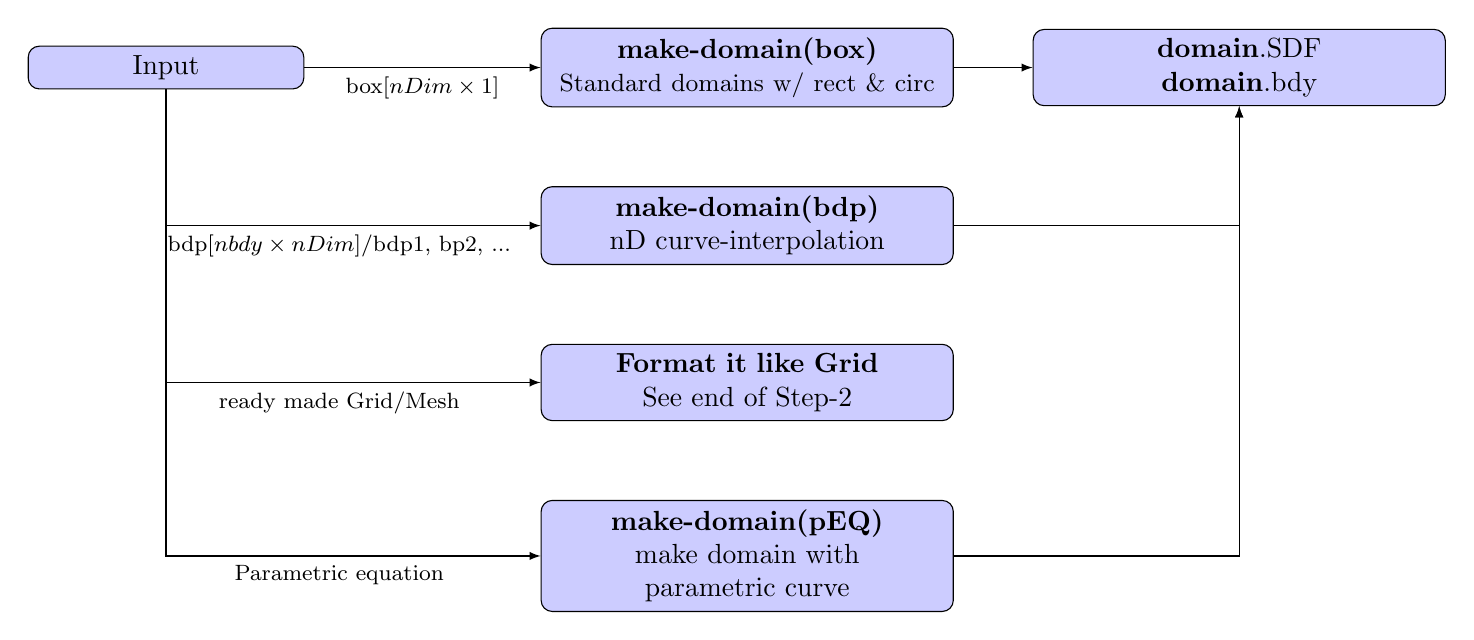
\begin{tikzpicture}[node distance=5.3cm]
        \node[block]                  (usr0){Input};
        \node[block, text width=5cm, right=3cm of usr0](usr2){\textbf{make-domain(box)}\\ \small Standard domains w/                                                          rect \& circ};
        \node[block,text width=5cm, below=1cm of usr2]   (usr1){\textbf{make-domain(bdp)}\\ nD curve-interpolation};
        \node[block,text width=5cm, below=1cm of usr1]   (usr3){\textbf{Format it like Grid} \\ See end of Step-2};
        \node[block,text width=5cm, right=1cm of usr2]   (domain){\textbf{domain}.SDF\\ \textbf{domain}.bdy};
        \node[block,text width=5cm, below=1cm of usr3]   (usr4){\textbf{make-domain(pEQ)}\\ make domain with parametric curve};

        \path[line] (usr0) --  node[below]{\footnotesize box[$nDim\times 1$]}        (usr2);
        \path[line] (usr0)  |-  node[below, xshift=2.2cm]{\footnotesize bdp[$nbdy\times nDim$]/bdp1, bp2, ...}        (usr1);
        \path[line] (usr0)  |-  node[below, xshift=2.2cm]{\footnotesize ready made Grid/Mesh }        (usr3);
        \path[line] (usr0)  |-  node[below, xshift=2.2cm]{\footnotesize Parametric equation }         (usr4);
        \path[line] (usr2) -- (domain); 
        \path[line] (usr1) -| (domain);
        \path[line] (usr4) -| (domain);
    
      \end{tikzpicture}%
}      
\end{center}
\end{frame}
%% ===========================================
\begin{frame}
\frametitle{\normalsize Step 2 --- Grid}
\begin{center}
\scalebox{0.6}{
      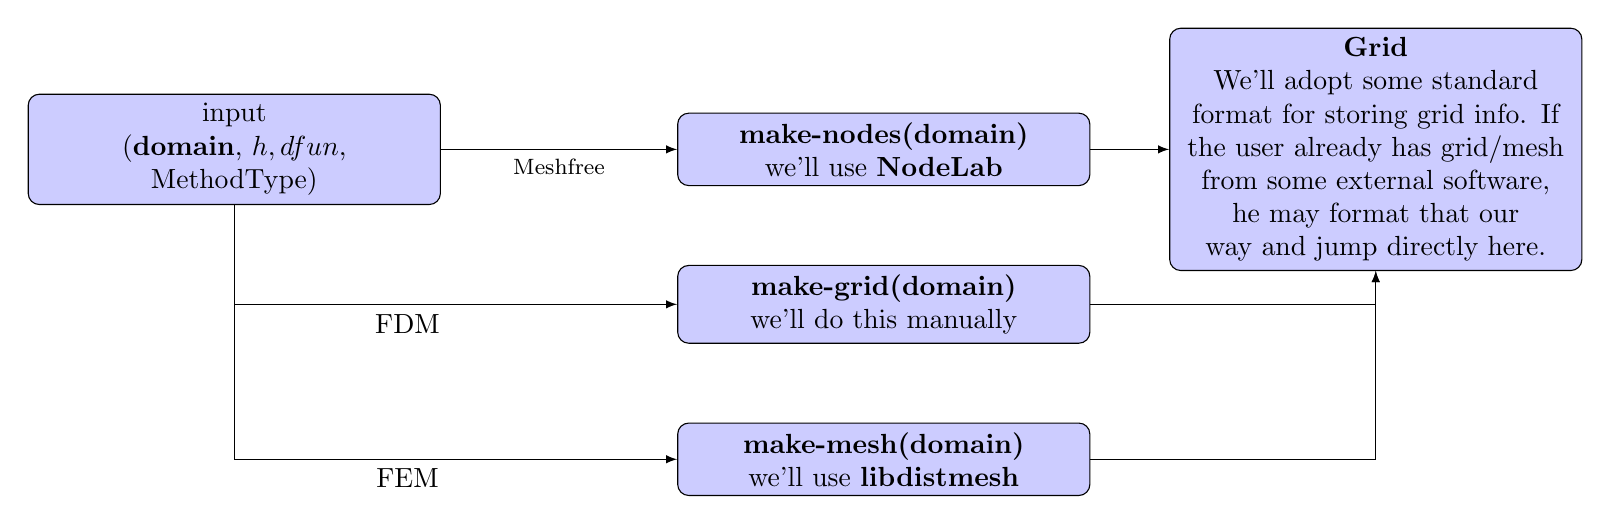
\begin{tikzpicture}[node distance=5.3cm]
        \node[block,text width=5cm] (usr0){input\\ (\textbf{domain}, $h,dfun$, MethodType)};
        \node[block, text width=5cm, right=3cm of usr0](usr2){\textbf{make-nodes(domain)}\\ we'll use \textbf{NodeLab}};
        \node[block,text width=5cm, below=1cm of usr2]   (usr1){\textbf{make-grid(domain)}\\ we'll do this manually};
        \node[block,text width=5cm, below=1cm of usr1]   (usr3){\textbf{make-mesh(domain)} \\ we'll use \textbf{libdistmesh}};
        \node[block,text width=5cm, right=1cm of usr2]   (grid){\textbf{Grid}\\ We'll adopt some standard format for storing grid info. If the user already has grid/mesh from some external software, he may format that our way and jump directly here.};
        

        \path[line] (usr0) --  node[below]{\footnotesize Meshfree}        (usr2);
        \path[line] (usr0)  |-  node[below, xshift=2.2cm]{FDM}        (usr1);
        \path[line] (usr0)  |-  node[below, xshift=2.2cm]{FEM}        (usr3);
        \path[line] (usr2) -- (grid); 
        \path[line] (usr1) -| (grid);
        \path[line] (usr3) -| (grid);
    
      \end{tikzpicture}%
}      
\end{center}
\end{frame}
%% ===========================================
%% ===========================================

\begin{frame}
\frametitle{\normalsize Step 3 --- Domain Decomposition \& Parallel Helpers}
\begin{center}
\scalebox{0.6}{
      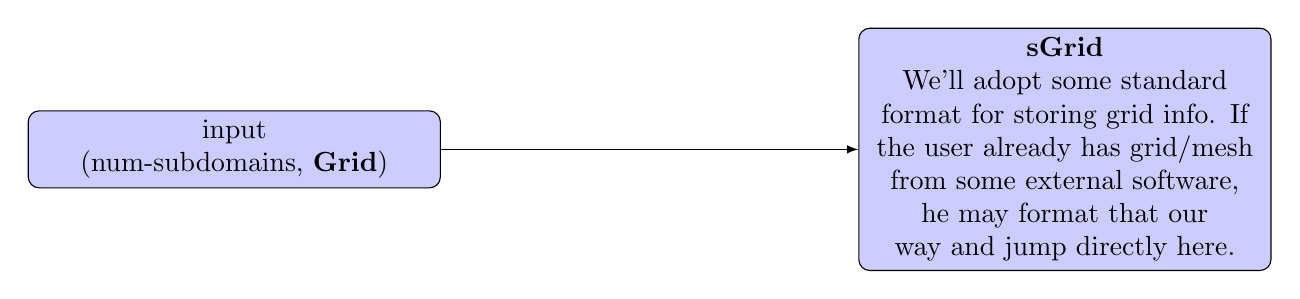
\begin{tikzpicture}[node distance=5.3cm]
        \node[block,text width=5cm] (usr0){input\\ (num-subdomains, \textbf{Grid})};
        \node[block,text width=5cm, right=5.3cm of usr0]   (sGrid){\textbf{sGrid}\\ We'll adopt some standard format for storing grid info. If the user already has grid/mesh from some external software, he may format that our way and jump directly here.};
        

       
        \path[line] (usr0) -- (sGrid); 
       
    
      \end{tikzpicture}%
}      
\end{center}
\end{frame}

%% ===========================================
%% ===========================================
\begin{frame}
\frametitle{\normalsize Step 4 --- Waveform Relaxation Class}

\end{frame}

%% ===========================================
%% ===========================================
\section{Second Section}
%% ===========================================
%% ===========================================

\begin{frame}
\frametitle{Table}
\begin{table}[H] % Option 'H' means you want the table (or figure) [exactly] HERE 
\begin{tabular}{l l l} \hline
\textbf{Treatments} & \textbf{Response 1} & \textbf{Response 2}\\ \hline \hline
Treatment 1 & 0.0003262 & 0.562 \\
Treatment 2 & 0.0015681 & 0.910 \\
Treatment 3 & 0.0009271 & 0.296 \\ \hline
\end{tabular}
\caption{Table caption}
\end{table}

\end{frame}

%% ===========================================
%% ===========================================

\begin{frame}
\frametitle{Theorem}
\begin{theorem}[Mass--energy equivalence]
$E = mc^2$
\end{theorem}
\end{frame}

%% ===========================================
%% ===========================================

\begin{frame}[fragile] % Need to use the fragile option when verbatim is used in the slide
\frametitle{Verbatim}
\begin{example}[Theorem Slide Code]
\begin{verbatim}
\begin{frame}
\frametitle{Theorem}
\begin{theorem}[Mass--energy equivalence]
$E = mc^2$
\end{theorem}
\end{frame}\end{verbatim}
\end{example}
\end{frame}

%% ===========================================
%% ===========================================

\begin{frame}
\frametitle{Figure}
Uncomment the code on this slide to include your own image from the same directory as the template .TeX file.
%\begin{figure}
%\includegraphics[width=0.8\linewidth]{test}
%\end{figure}
\end{frame}

%% ===========================================
%% ===========================================

\begin{frame}[fragile] % Need to use the fragile option when verbatim is used in the slide
\frametitle{Citation}
An example of the \verb|\cite| command to cite within the presentation:\\~

This statement requires citation \cite{p1}.
\end{frame}

%% ===========================================
%% ===========================================

\begin{frame}
\frametitle{References}
\footnotesize{
\begin{thebibliography}{99} % Beamer does not support BibTeX so references must be inserted manually as below
\bibitem[Smith, 2012]{p1} John Smith (2012)
\newblock Title of the publication
\newblock \emph{Journal Name} 12(3), 45 -- 678.
\end{thebibliography}
}
\end{frame}

%% ===========================================
%% ===========================================

\begin{frame}
\Huge{\centerline{The End}}
\end{frame}

%% ===========================================
%% ===========================================

\end{document}
